上一节讨论的是在同一台机器上运行多个线程,而这些线程之间没有任何交互。如果能够以一种方式将程序所做的工作分割到多个线程之间,那么无论如何都要这样做。

线程之间通常必须交互,因为它们正在为一个共同的结果工作。这种交互是通过线程之间,通过共享资源(内存)进行通信的方式进行的。我们现在必须理解这对性能的影响。

从一个简单的例子开始。假设我们要计算多个值的和,有很多数字要加,但最后只有一个结果。有很多数字需要相加,所以我们想要在几个线程之间进行添加工作。但是只有一个结果,因此线程在做加和时,这个值时必须进行交互。

\hspace*{\fill} \\ %插入空行
\noindent
\textbf{02\_sharing\_incr.C}
\begin{lstlisting}[style=styleCXX]
unsigned long x {0};
void BM_incr(benchmark::State& state) {
	for (auto _ : state) {
		benchmark::DoNotOptimize(++x);
	}
}
BENCHMARK(BM_incr)->Threads(2);
\end{lstlisting}

为了简单起见,我们总是将结果递增1(整数相加的代价与值无关,并且不想对不同值的生成进行基准测试,而只想对加法本身进行基准测试)。由于基准函数由每个线程调用,因此在这个函数中声明的任何变量都独立存在于每个线程的堆栈上,这些变量不共享。为了得到两个线程都参与的共同结果,变量必须在基准函数之外的文件范围内声明(这是个坏主意,但在微基准的非常有限的上下文中是必要和可接受的)。

当然,这个程序有一个比全局变量更大的问题:这是个错误的程序,其结果未定义。我们有两个线程递增相同的值,增加一个值需要3个步骤:程序从内存中读取值,在寄存器中增加值,然后将新值写回内存。两个线程完全可以同时读取相同的值(0),在每个处理器(1)上分别递增,然后写回。写第二个线程的线程只是重写第一个线程的结果,在两次增量之后,结果是1,而不是2。这是因为两个线程为了写入同一内存位置而进行了竞争,这种竞争称为\textbf{数据竞争}。

既然已经理解了为什么这种无保护的并发访问会出问题,那么最好忘记它。相反,请遵循这个一般的规则:如果在没有同步的情况下,让多个线程访问相同的内存位置,并且这些访问中有一个是写操作,则会出现未定义的结果。这是非常重要的,没有必要确切地指出必须发生哪些操作序列会得到不正确的结果。事实上,在这种推理过程中什么也得不到。当有两个或更多的线程访问同一个内存位置时,就会遇到数据竞争,除非能保证以下两件事中的一件:要么所有的访问都是只读的,要么所有的访问都使用了正确的内存同步(这一点我们还没有了解)。

计算求和的问题要求我们将结果写入结果变量,所以访问肯定不是只读的。内存访问的同步通常由互斥锁提供,每次访问线程间共享的变量都必须由互斥锁保护(当然,所有线程的互斥锁必须相同)。

\hspace*{\fill} \\ %插入空行
\noindent
\textbf{03\_mutex\_incr.C}
\begin{lstlisting}[style=styleCXX]
unsigned long x {0};
std::mutex m;

{ // Concurrent access happens here
	std::lock_guard<std::mutex> guard(m);
	++x;
}
\end{lstlisting}

\texttt{lock\_guard}锁在其构造函数中锁定互斥锁,并在析构函数解锁。一次只有一个线程可以拥有锁,这样就可以对共享结果变量进行增加数值的操作。这时,其他线程被锁阻塞,直到第一个线程释放锁后,才能获取锁。注意,只要至少有一个线程在修改变量,所有的访问(包括读和写)都必须被阻塞。

锁是确保多线程程序正确性的最简单方法,但就性能而言,它还挺难研究的。锁的实现相当复杂,会经常涉及系统调用。我们将从一个同步选项开始,在这个特定的例子中,这个方式会更容易分析:原子变量。

C++提供了一个将变量声明为原子变量的选项。这意味着对这个变量支持的所有操作都是不可中断的原子事务执行的:任何观察这个变量的其他线程都将在原子操作之前或之后看到它的状态,但绝不会在操作的中间看到它的状态。例如,C++中所有的整数原子变量都支持原子增量操作:如果一个线程正在执行这个操作,那么在第一个操作完成之前,其他线程都不能访问这个变量。这些操作需要一定的硬件支持,例如:原子增量是一种特殊的硬件指令,它读取旧的值,增加它的值,然后写入新值,所有这些都作为一个单独的硬件操作。

我们的示例中,只需要一个原子自增。必须强调的是,无论我们决定使用什么同步机制,所有线程都必须使用相同的机制来并发访问特定的内存位置。如果我们在一个线程上使用原子操作,只要所有线程都使用原子操作,从而保证没有数据竞争。如果另一个线程使用互斥锁或非原子访问,那之前的保证就都没用了,从而结果依旧是未定义的。

用C++的原子操作重写我们的基准测试:

\hspace*{\fill} \\ %插入空行
\noindent
\textbf{02\_sharing\_incr.C}
\begin{lstlisting}[style=styleCXX]
std::atomic<unsigned long> x(0);
void BM_shared(benchmark::State& state) {
	for (auto _ : state) {
		benchmark::DoNotOptimize(++x);
	}
}
\end{lstlisting}

程序现在是正确的:这里没有数据竞争。这并不一定准确,因为单个自增是一个非常短的时间间隔来,我们真的应该手动展开循环或使用宏,并在每次循环迭代中进行多次递增(我们已经在上一章中做了这一点,所以可以在那里看到宏)。让我们看看它的表现如何。如果线程之间没有交互,两个线程计算总和的时间将是一个线程计算总和的一半:

%\hspace*{\fill} \\ %插入空行
\begin{center}
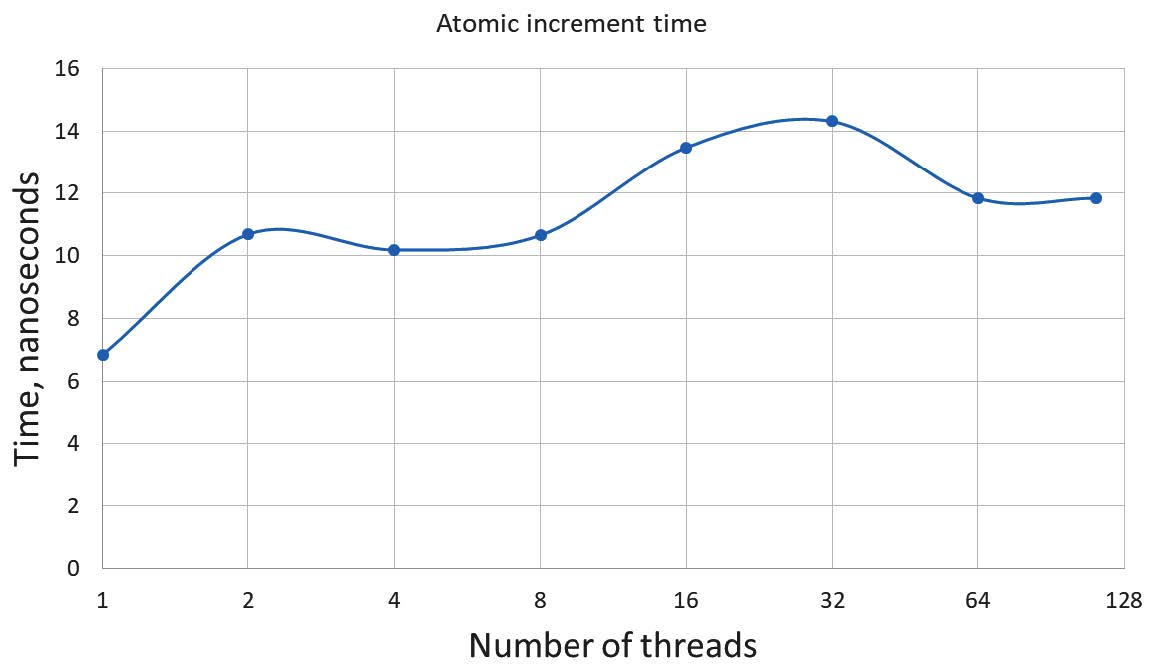
\includegraphics[width=0.9\textwidth]{content/1/chapter5/images/4.jpg}\\
图5.4 - 多线程程序中的原子自增时间
\end{center}

我们对结果进行了标准化,以显示单个增量的平均时间,即计算和除以相加总数的时间。这个程序的性能非常令人失望:不仅没有任何改进,在两个线程上计算总和要比在一个线程上花费更长的时间。

如果我们使用互斥锁,结果会更糟:

%\hspace*{\fill} \\ %插入空行
\begin{center}
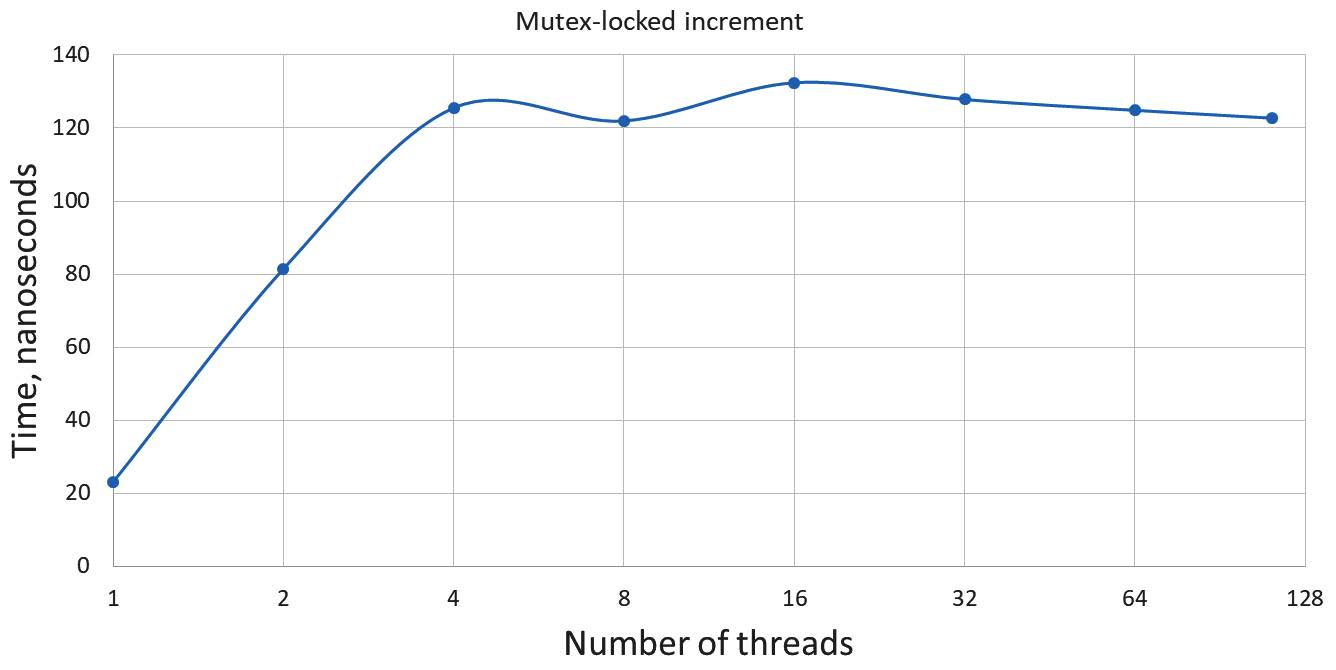
\includegraphics[width=0.9\textwidth]{content/1/chapter5/images/5.jpg}\\
图5.5 - 在多线程程序中使用互斥量会增加耗时
\end{center}

首先,正如我们所预料的那样,锁定互斥锁是一个相当耗时的操作,即使是在一个线程上:互斥锁是23纳秒,而原子变量是7纳秒。随着线程数量的增加,性能下降得更快。

可以从这些实验中学到很多。程序中访问共享数据的部分永远不会扩展,访问共享数据的最佳性能是单线程性能。当有两个或更多的线程同时访问相同的数据,性能只会变得更糟。当然,如果两个线程在不同的时间访问相同的数据,它们实际上不会相互交互,因此两次都获得了单线程性能。多线程程序的性能优势来自于线程独立进行的计算,而不需要同步。根据定义,这样的计算可以在不共享的数据上进行(无论如何,若希望程序结果正确)。但是为什么对共享数据的并发访问有如此开销呢?下一节中,我们将了解其中原因。我们也将了解如何详细的解析测量结果。








